\section{Zeitlicher Ablauf}

Im Großen und Ganzen hat sich die Zeitplanung aus der Entwurfsphase bewährt. Die Aufteilung in Aufgabenbereiche wurde weitgehend eingehalten. Während der Entwicklung hat sich als vorteilhaft erwiesen, eng ineinandergreifende Komponenten parallel zu Entwickeln, um den geschriebenen Code sofort testen zu können. Im aktualisierten Gantt-Diagramm erscheinen deshalb einige Einheiten deutlich größer. Tatsächlich hat sich aus der parallelisierung kein höherer Zeitaufwand ergeben. Trotzdem haben sich einige kleinere Änderungen im Laufe der Implementierungsphase ergeben, welche im Folgenden genauer dargestellt werden.

\subsection{Build-System}
Die Inbetriebnahme der Build-Systems sowie des Continous-Integration-Servers hat sich aufgrund einiger Schwierigkeiten bei der Konfiguration um einige Tag in die Weihnachtsferien hinein verschoben.

\subsection{Stubs und Unit-Tests}
Ursprünglich war geplant, vor der eigentlichen Implementierung Unit-Tests zu erstellen und dementsprechend die Klassen mit Stubs auszurüsten, welche die Tests erfolgreich ablaufen lassen. Da das Parsen von Testprogrammen jedoch bereits frühzeitig möglich war wurden stattdessen parallel zur Implementierung Unit-Tests mit an den Testfall angepassten Testprogrammen geschrieben.

\subsection{Parser}
Aufgrund der Entscheidung, keine eigene Schnittstellenklasse zum Parser zu implementieren (siehe \ref{aenderung_parser}), sondern die von ANTLR generierte Klasse direkt zu verwenden, entfiel diese Aufgabe.

\subsection{Beweiserschnittstelle}
Die Abhängigkeit zwischen der Z3-Anbindung und des SMTLIB-Compilers wurde aufgelöst, da es sich als vorteilhaft herausstellte, beide Tasks parallel zu entwickeln.

\subsection{Interpreter}
Der Entschluss, alle Debug-Logik in einer seperaten "Debugger"-Komponente zu implementieren (siehe \ref{aenderung_interpreter_breakpoints}), führte dazu, dass die Einheit "Breakpoints" vom Aufgabenbereich "Interpreter" in den Aufgabenbereich der GUI-Entwicklers verschoben wurde.

\begin{landscape}%
	\begin{figure}%
		\vspace{-2cm}
		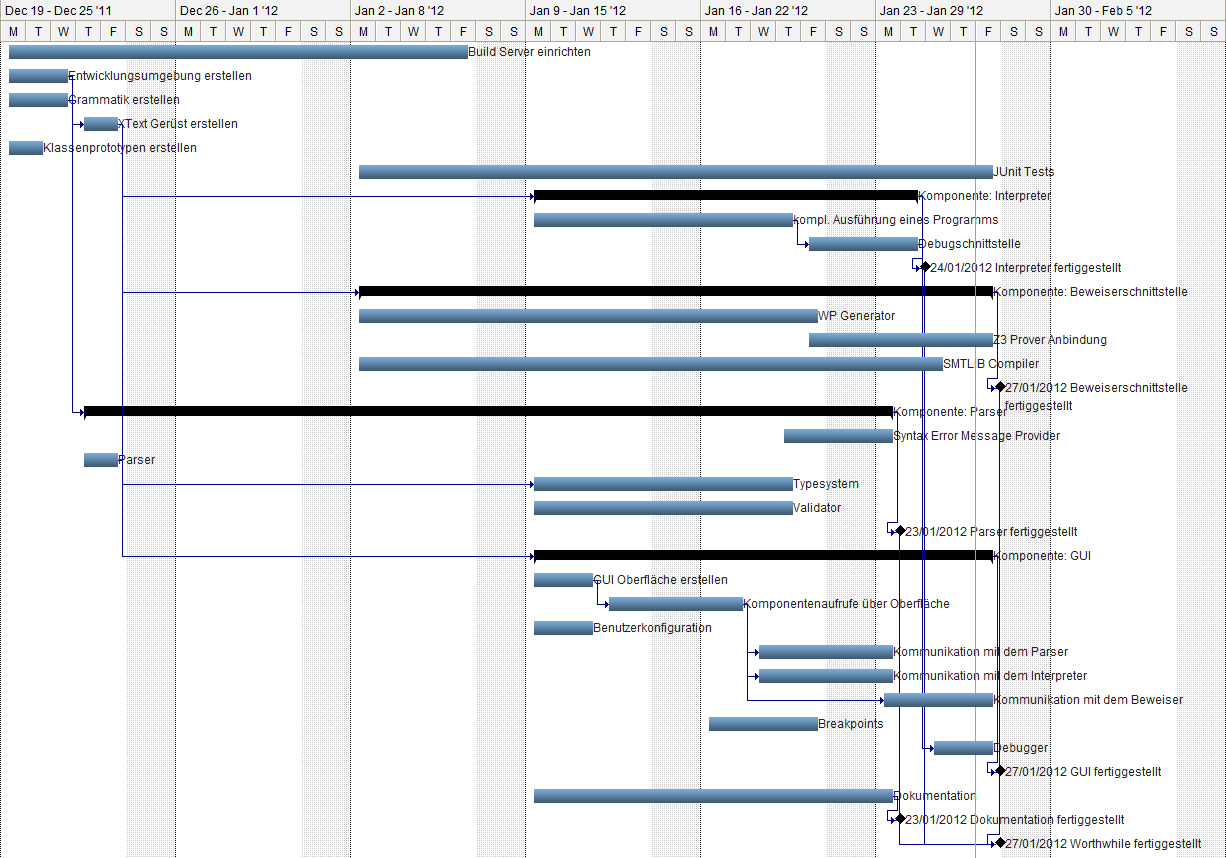
\includegraphics[height=1.2\textheight]{images/gantt_implementierung_diag.png}%
		\caption{Tatsächlicher Ablauf der Implementierungsphase.}%
	\end{figure}%
\end{landscape}
